La curva $C$ recorre positivamente el polígono mostrado. Use el teorema de Green para calcular
\[
\oint_C-y\,dx+x\,dy.
\]
\begingroup
\shorthandoff{>}
\begin{center}
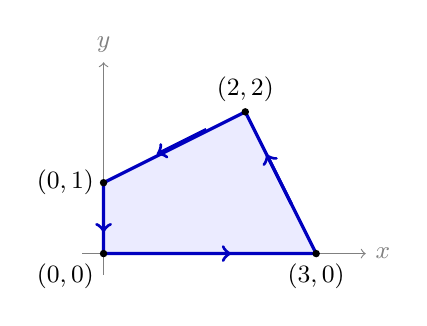
\begin{tikzpicture}[scale=.9,every node/.style={font=\small}]
    \draw[->,gray] (-.3,0)--(3.7,0) node[right] {$x$};
    \draw[->,gray] (0,-.3)--(0,2.7) node[above] {$y$};
    \fill[blue!8] (0,0)--(3,0)--(2,2)--(0,1)--cycle;
    \draw[blue!75!black,very thick] (0,0)--(3,0)--(2,2)--(0,1)--cycle;
    \draw[->,blue!75!black,very thick] (1,0)--(1.8,0);
    \draw[->,blue!75!black,very thick] (2.65,.7)--(2.3,1.4);
    \draw[->,blue!75!black,very thick] (1.45,1.75)--(.75,1.4);
    \draw[->,blue!75!black,very thick] (0,.75)--(0,.3);
    \fill (0,0) circle (1.5pt) node[below left] {$(0,0)$};
    \fill (3,0) circle (1.5pt) node[below] {$(3,0)$};
    \fill (2,2) circle (1.5pt) node[above] {$(2,2)$};
    \fill (0,1) circle (1.5pt) node[left] {$(0,1)$};
\end{tikzpicture}
\end{center}
\endgroup
